% CV template – photo & profil moved to right column
\documentclass{article}
% Encoding & core font
\usepackage[T1]{fontenc}
\usepackage[utf8]{inputenc}
\usepackage{textcomp}
\usepackage{times}
\usepackage{newtxtext} % Times‑compatible extended glyph set

% Layout
\usepackage{geometry}
\geometry{a4paper,left=0.6cm,right=0.7cm,top=1cm,bottom=1cm,columnsep=0.8cm}

% Core packages
\usepackage{fontawesome}
\usepackage[hidelinks]{hyperref}
\usepackage{multicol,paracol,tikz,adjustbox,tabularx,xcolor,enumitem}
\usepackage{ragged2e}
\newcolumntype{Y}{>{\RaggedRight\arraybackslash}X}
\setlist[itemize]{itemsep=1pt,leftmargin=*,topsep=-10pt}

% Colors
\definecolor{maincolor}{HTML}{ffffff}
\definecolor{seccolor}{HTML}{0b1f3b}
\definecolor{gray}{HTML}{8c94a9}
\definecolor{sidetext}{HTML}{59cee5}
\definecolor{Green}{HTML}{2caf00}
\definecolor{lightgray}{HTML}{D3D3D3}

% --- Side blue band ---------------------------------------------------
\usepackage{eso-pic}
\AddToShipoutPictureBG{%% background split in 70/30
  \begin{tikzpicture}[remember picture,overlay]
    \fill[seccolor] (0.7\paperwidth,0) rectangle (\paperwidth,\paperheight);
    \fill[maincolor] (0,0) rectangle (0.7\paperwidth,\paperheight);
  \end{tikzpicture}}

% ----------------------------------------------------------------------
\setlength{\parindent}{0pt}
\newcommand{\cvsection}[1]{%
  \par\bigskip
  {\bfseries\Large #1}\par
  \noindent\rule{\linewidth}{0.8pt}\par\medskip}

% Document -------------------------------------------------------------
\begin{document}\pagestyle{empty}
\columnratio{0.7}\begin{paracol}{2}

% ===================== LEFT COLUMN (70 %) =============================
{\LARGE\textbf{Judikael Mourouvin}}

\bigskip
{\large\textbf{Technicien support informatique \& marketing digital}}

\vspace{0.8cm}

\cvsection{EXPÉRIENCE}
\colorbox{maincolor}{%
  \begin{minipage}{\linewidth}
    \noindent
    \textbf{Alternant en marketing digital}\hfill 09/2023 - 08/2024\\
    Mairie du Gosier – DSI\\[-0.3em]
    \begin{itemize}[leftmargin=*]
      \item Pilotage de projets numériques : analyse des besoins, déploiement et suivi. \item Support N1/N2 et formation des agents aux outils collaboratifs. \item Contribution aux campagnes de communication digitale de la collectivité.
    \end{itemize}
  \end{minipage}}

\vspace{3mm}

\colorbox{maincolor}{%
  \begin{minipage}{\linewidth}
    \noindent
    \textbf{Animateur de la zone informatique}\hfill 10/2022 - 09/2023\\
    Pôle Emploi – Gosier\\[-0.3em]
    \begin{itemize}[leftmargin=*]
      \item Assistance quotidienne des usagers ; diminution des incidents récurrents. \item Maintenance et configuration du parc (≈25 postes, imprimantes, réseau local). \item Diagnostic et résolution de pannes matériel/logiciel (délai moyen < 24 h).
    \end{itemize}
  \end{minipage}}

\vspace{3mm}

\colorbox{maincolor}{%
  \begin{minipage}{\linewidth}
    \noindent
    \textbf{Stagiaire informaticien}\hfill 05/2020 - 08/2021\\
    Numerika – Baie-Mahault\\[-0.3em]
    \begin{itemize}[leftmargin=*]
      \item Installation et maintenance des postes et périphériques. \item Support de proximité (taux de résolution : 95 \%).
    \end{itemize}
  \end{minipage}}

\cvsection{FORMATION}
\colorbox{maincolor}{%
  \begin{minipage}{\linewidth}
    \noindent
    \textbf{Bachelor Marketing Digital}\hfill 09/2023 - 08/2024\\
    CFA IUTS\\[-0.3em]
    \begin{itemize}[leftmargin=*]
      \item SEO/SEA, réseaux sociaux, analyse de données \item Gestion de campagnes et projets e-commerce
    \end{itemize}
  \end{minipage}}

\vspace{3mm}

\colorbox{maincolor}{%
  \begin{minipage}{\linewidth}
    \noindent
    \textbf{BTS Systèmes Numériques option Informatique \& Réseaux}\hfill 09/2019 - 06/2021\\
    Lycée de Chevalier Saint-Georges, Abymes\\[-0.3em]
    \begin{itemize}[leftmargin=*]
      \item Architecture réseau et sécurité \item Programmation embarquée, support et maintenance
    \end{itemize}
  \end{minipage}}

% ===================== RIGHT COLUMN (30 %) ============================
\switchcolumn\color{white}\hspace*{0.4cm}\begin{minipage}{0.88\linewidth}

% ---- Photo -----------------------------------------------------------
\centering
\ifx\relax214fd333fa9540668d03fc866dd702b6.png\relax\else
  \begin{tikzpicture}
    \clip (0,0) circle (1.8cm) node[anchor=center]
          {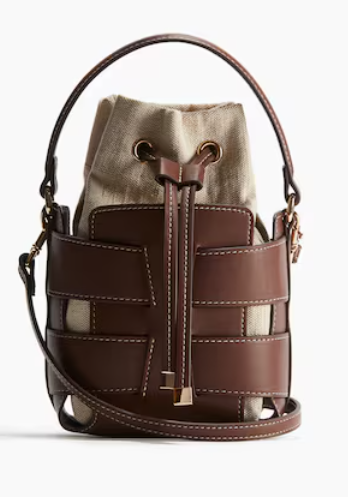
\includegraphics[width=0.5\textwidth]{214fd333fa9540668d03fc866dd702b6.png}};
  \end{tikzpicture}
\fi

% ---- Profile (Résumé) ------------------------------------------------
\cvsection{PROFIL}
\begingroup           % ouvre un groupe local
\justifying         % rétablit la justification pleine
  Technicien polyvalent, j’allie expertise en support informatique (mise en service, maintenance, assistance N1/N2) et maîtrise des leviers du marketing digital (SEO, réseaux sociaux, campagnes). Curieux, organisé et orienté utilisateur, j’ai optimisé la satisfaction des agents de la Mairie du Gosier tout en contribuant à la visibilité en ligne de la collectivité. Je souhaite désormais mettre ces compétences au profit d’une structure ambitieuse pour accélérer ses projets numériques.
\endgroup             % referme : on revient à \raggedright

% ---- Contact ---------------------------------------------------------
\cvsection{CONTACT}
\begin{tabular}{@{}c l}
  \faPhone & \href{tel:+590 0690 91 14 48}{+590 0690 91 14 48} \\[2pt]
  \faEnvelope & \href{mailto:jkmou971@gmail.com}{jkmou971@gmail.com} \\[2pt]
  \faMapMarker & 97190 Gosier \\[2pt]
  \faLinkedin & \href{}{}
\end{tabular}
\vspace{0.2cm}
% ---- Skills ----------------------------------------------------------
\cvsection{COMPÉTENCES}
\begin{itemize}[leftmargin=*]
\item Administration
\item Réseaux
\item Support
\item Maintenance
\item Diagnostic
\item Marketing
\item Configuration\end{itemize}
\vspace{0.2cm}
% ---- Languages -------------------------------------------------------
\cvsection{LANGUES}
\begin{itemize}[leftmargin=*]
\item English - \textcolor{gray}{Intermédiaire}
\item Espagnol - \textcolor{gray}{Notions}\end{itemize}
\vspace{0.2cm}
% ---- Interests -------------------------------------------------------
\cvsection{INTÉRÊTS}
\begin{itemize}[leftmargin=*]
\item Lecture
\item Sport
\item Musique
\item Voyage
\end{itemize}

\end{minipage}
\end{paracol}
\end{document}
